\documentclass[11pt,a4paper]{article}

% =============================================================================
% 1. PACKAGES (DO NOT EDIT)
% =============================================================================
\usepackage[utf8]{inputenc}
\usepackage[T1]{fontenc}
\usepackage{lmodern}
\usepackage[a4paper, top=3.5cm, bottom=2.5cm, left=2.5cm, right=2.5cm, headheight=42pt, headsep=1.0cm]{geometry}
\usepackage{longtable}
\usepackage{float}
\usepackage{tikz}
\usetikzlibrary{arrows.meta,positioning,fit,backgrounds,calc}
\usepackage[table]{xcolor}
\usepackage{tabularx}
\usepackage{array}
\usepackage{fancyhdr}
\usepackage{graphicx}
\usepackage{amsmath}
\usepackage[hidelinks]{hyperref}

% =============================================================================
% 2. DOCUMENT METADATA
% (Values entered here will automatically populate Page 1 and all page headers)
% =============================================================================
\newcommand{\Organization}{HSB}
\newcommand{\ProjectName}{EWAS}
\newcommand{\DocTitle}{Ground Segment - Design Definition File}
\newcommand{\DocNumber}{EWAS-HSB-GSEG-DDF-03} % Suffix 03 retained pending owner confirmation.
\newcommand{\DocIssue}{0.1}                  % Working draft; no approval recorded.
\newcommand{\DocDate}{}                     % Issue date pending owner confirmation.
\newcommand{\CINumber}{02}                  % Ground Segment CI-02.

% =============================================================================
% 3. COLORS AND TEMPLATE STYLING (DO NOT EDIT)
% =============================================================================
\definecolor{TitleBlue}{HTML}{1F497D}         % Main title color on Page 1
\definecolor{HeadingBlue}{HTML}{365F91}       % Section heading color (H1)
\definecolor{SubHeadingBlue}{HTML}{4F81BD}    % Subsection heading (H2) and rule color
\definecolor{TableHeaderBlue}{HTML}{4F81BD}   % Table header background color
\definecolor{TableRowLightBlue}{HTML}{DBE5F1} % Alternating table row background color
\definecolor{TableBorderBlue}{HTML}{95B3D7}   % Styled table border color

% Paragraph settings
\setlength{\parindent}{0pt}
\setlength{\parskip}{0.6em}

% Disable section numbering (matching the PDF template) while keeping TOC entries.
% To enable section numbering (e.g., 1, 1.1), change -1 to 3.
\setcounter{secnumdepth}{-1}
\setcounter{tocdepth}{2}

% Section, subsection, and list title styling
\makeatletter
\renewcommand\section{\@startsection{section}{1}{\z@}%
    {-3.0ex \@plus -1ex \@minus -.2ex}%
    {1.5ex \@plus .2ex}%
    {\normalfont\Large\bfseries\sffamily\color{HeadingBlue}}}

\renewcommand\subsection{\@startsection{subsection}{2}{\z@}%
    {-2.5ex \@plus -1ex \@minus -.2ex}%
    {1.0ex \@plus .2ex}%
    {\normalfont\large\bfseries\sffamily\color{SubHeadingBlue}}}

\renewcommand\subsubsection{\@startsection{subsubsection}{3}{\z@}%
    {-2.0ex \@plus -1ex \@minus -.2ex}%
    {0.8ex \@plus .2ex}%
    {\normalfont\normalsize\bfseries\sffamily\color{SubHeadingBlue}}}

% Dotted leaders in the Table of Contents for top-level sections as well
\renewcommand*\l@section{\@dottedtocline{1}{0em}{1.5em}}
\renewcommand*\l@subsection{\@dottedtocline{2}{1.5em}{2.3em}}

% Centered blue headings for Table of Contents, List of Tables, and List of Figures
\renewcommand{\contentsname}{Table of Contents}
\renewcommand{\listtablename}{List of Tables}
\renewcommand{\listfigurename}{List of Figures}

\renewcommand\tableofcontents{
    {\centering\normalfont\Large\bfseries\sffamily\color{HeadingBlue}\contentsname\par}
    \vspace{0.8em}
    \@starttoc{toc}
}
\renewcommand\listoftables{
    {\centering\normalfont\Large\bfseries\sffamily\color{HeadingBlue}\listtablename\par}
    \vspace{0.8em}
    \@starttoc{lot}
}
\renewcommand\listoffigures{
    {\centering\normalfont\Large\bfseries\sffamily\color{HeadingBlue}\listfigurename\par}
    \vspace{0.8em}
    \@starttoc{lof}
}
\makeatother

% Helper macros
\newcommand{\thead}[1]{\textcolor{white}{\textbf{\textsf{#1}}}}
\providecommand{\abbr}[1]{#1}

% =============================================================================
% 4. HEADER AND FOOTER (WITH UNIVERSITY LOGOS)
% =============================================================================
\pagestyle{fancy}
\fancyhf{}
\renewcommand{\headrulewidth}{0pt}
\renewcommand{\footrulewidth}{0pt}

\fancyhead[L]{
    \raisebox{-0.5\height}{
\includegraphics[height=1.05cm]{figs/hsb_logo.png}}
}
\fancyhead[C]{
    {\small\textbf{Early Warning Alarm System (\abbr{EWAS})}}
}
\fancyhead[R]{
    \raisebox{-0.5\height}{
\includegraphics[height=1.2cm]{figs/pg_logo.jpg}}
}
\fancyfoot[R]{\thepage}

% Style for Page 1 (logos in top corners, no page number in footer)
\fancypagestyle{firstpage}{
    \fancyhf{}
    \renewcommand{\headrulewidth}{0pt}
    \renewcommand{\footrulewidth}{0pt}
    \fancyhead[L]{\raisebox{-0.5\height}{
\includegraphics[height=1.05cm]{figs/hsb_logo.png}}}
    \fancyhead[R]{\raisebox{-0.5\height}{
\includegraphics[height=1.2cm]{figs/pg_logo.jpg}}}
}

% =============================================================================
% DOCUMENT BODY
% =============================================================================
\begin{document}

% -----------------------------------------------------------------------------
% PAGE 1: TITLE PAGE & DOCUMENT INFORMATION
% -----------------------------------------------------------------------------
\thispagestyle{firstpage} % Use \thispagestyle{empty} if you do not want logos on Page 1
\phantomsection
\addcontentsline{toc}{section}{Document Information}

\begin{center}
    {\large \ProjectName}
\end{center}

\vspace*{5.5cm}

\begin{center}
    {\fontsize{24}{28}\selectfont\sffamily\color{TitleBlue}\DocTitle\par}
    \vspace{0.35cm}
    {\color{SubHeadingBlue}\hrule height 0.8pt}
\end{center}

\vfill

% --- HOW TO EDIT THE PAGE 1 TABLE ---
% Part 1 (first 4 rows): automatically populated from Section 2 at the top of the file.
% Part 2 (signatures & roles): enter data between the & symbols in the format:
%     {Full Name} & {Role Name} & {Signature/Date (or leave blank)} \\[1.2em] \hline
{\renewcommand{\arraystretch}{1.25}%
\arrayrulecolor{black}%
\noindent
\begin{tabularx}{\textwidth}{|X|X|}
    \hline
    Document Number & \DocNumber \\ \hline
    Issue           & \DocIssue{} (Draft) \\ \hline
    Issue Date      & \DocDate   \\ \hline
    CI Number       & \CINumber  \\
\end{tabularx}\par\nointerlineskip
\noindent
\begin{tabularx}{\textwidth}{|X|X|X|}
    \hline
    % COLUMN 1: Name             & COLUMN 2: Responsibility & COLUMN 3: Signature/Date
    Name                         & Responsibility           & Signature/Date                   \\ \hline
    Prepared by                  &                          &                                  \\ \hline
                                 &                          &                                  \\[1.2em] \hline
    Checked by                   &                          &                                  \\ \hline
                                 &                          &                                  \\[1.2em] \hline
    Approved by                  &                          &                                  \\ \hline
                                 &                          &                                  \\[1.2em] \hline
\end{tabularx}}

\newpage

% -----------------------------------------------------------------------------
% PAGE 2: DOCUMENT CHANGE RECORD
% -----------------------------------------------------------------------------
\section{Document Change Record}

% --- HOW TO EDIT THE DOCUMENT CHANGE RECORD TABLE ---
% Each row has 4 columns separated by &:
% \textbf{Issue} & {Date} & {Description} & {Sections Affected} \\ \hline
% To add a new row, copy the last line before \end{tabularx}.
{\renewcommand{\arraystretch}{1.25}%
\arrayrulecolor{TableBorderBlue}%
\rowcolors{2}{white}{TableRowLightBlue}%
\noindent
\begin{tabularx}{\textwidth}{|>{\raggedright\arraybackslash}p{2.0cm}|>{\raggedright\arraybackslash}p{2.5cm}|>{\raggedright\arraybackslash}X|>{\raggedright\arraybackslash}p{4.5cm}|}
    \hline
    \rowcolor{TableHeaderBlue}
    % COLUMN 1: Issue & COLUMN 2: Date  & COLUMN 3: Description      & COLUMN 4: Sections Affected
    \thead{Issue}     & \thead{Date}    & \thead{Description}        & \thead{Sections Affected}     \\ \hline
    \textbf{0.1} & & Working draft: template cleanup and addition of Section 4, Functional Description. & Document information; Section 4 \\ \hline
\end{tabularx}}

\newpage

% -----------------------------------------------------------------------------
% PAGE 3: TABLE OF CONTENTS, LIST OF TABLES, LIST OF FIGURES (AUTO-GENERATED)
% -----------------------------------------------------------------------------
\tableofcontents

\vspace{2.5cm}
\listoftables

\vspace{2.5cm}
\listoffigures

\newpage

% -----------------------------------------------------------------------------
% PAGE 4: REFERENCES (AD, RD, TERMS & ABBREVIATIONS)
% -----------------------------------------------------------------------------
\section{References}

\subsection{Applicable Documents (AD)}

% --- HOW TO EDIT THE APPLICABLE DOCUMENTS (AD) TABLE ---
% Columns are separated by &:
% \textbf{AD-XX} & {Document Number} & {Document Title} & {Issue} \\ \hline
{\renewcommand{\arraystretch}{1.25}%
\arrayrulecolor{TableBorderBlue}%
\rowcolors{2}{white}{TableRowLightBlue}%
\noindent
\begin{tabularx}{\textwidth}{|p{2.4cm}|p{3.6cm}|X|p{2.4cm}|}
    \hline
    \rowcolor{TableHeaderBlue}
    % COLUMN 1: AD No. & COLUMN 2: Document Number & COLUMN 3: Title         & COLUMN 4: Issue
    \thead{AD No.}     & \thead{Document Number}   & \thead{Title}           & \thead{Issue}     \\ \hline
\end{tabularx}}

\vspace{0.8em}
\subsection{Reference Documents (RD)}

% --- HOW TO EDIT THE REFERENCE DOCUMENTS (RD) TABLE ---
% Columns are separated by &:
% \textbf{RD-XX} & {Document Number} & {Document Title} & {Issue} \\ \hline
{\renewcommand{\arraystretch}{1.25}%
\arrayrulecolor{TableBorderBlue}%
\rowcolors{2}{white}{TableRowLightBlue}%
\noindent
\begin{tabularx}{\textwidth}{|p{2.4cm}|p{3.6cm}|X|p{2.4cm}|}
    \hline
    \rowcolor{TableHeaderBlue}
    % COLUMN 1: RD No. & COLUMN 2: Document Number & COLUMN 3: Title         & COLUMN 4: Issue
    \thead{RD No.}     & \thead{Document Number}   & \thead{Title}           & \thead{Issue}     \\ \hline
\end{tabularx}}

\vspace{0.8em}
\subsection{Terms, Definitions and Abbreviations}

% --- HOW TO EDIT THE ABBREVIATIONS TABLE ---
% Columns are separated by &:
% \textbf{ABBREVIATION} & {Full Meaning / Definition} \\ \hline
{\renewcommand{\arraystretch}{1.25}%
\arrayrulecolor{TableBorderBlue}%
\rowcolors{2}{white}{TableRowLightBlue}%
\noindent
\begin{tabularx}{\textwidth}{|X|X|}
    \hline
    \rowcolor{TableHeaderBlue}
    % COLUMN 1: Abbreviation          & COLUMN 2: Meaning
    \thead{Abbreviation}              & \thead{Meaning}                                   \\ \hline
    \textbf{ECSS}                     & European Cooperation for Space Standardization    \\ \hline
    \textbf{CI}                       & Configuration Item                                \\ \hline
\end{tabularx}}

\newpage

% Sections 1--3 will be added after their content is supplied and reviewed.

% GSEG DDF — Section 4, concise English working draft.
% Content only. Required packages in DDFmain.tex: longtable, tikz, float.
% TikZ libraries: arrows.meta, positioning, fit.
% Manual section numbers match the existing GSEG TRS/DDF style (secnumdepth=-1).
\section{4. Functional Description}

\subsection{4.1 Functional Architecture}

The Ground Segment (GSEG, CI-02) integrates seven subsystems: Ground Station Network (GSN), Command \& Control (C\&C), Data Processing System (DPS), Early Warning System (EWS), Mission Control Center (MCC), Data Archiving System (DAS), and Ground Infrastructure Subsystem (GIS). Its time-critical event-response chain uses GSN, C\&C, DPS and EWS. MCC supervises operations, owns flight dynamics and mission planning, and supports authorized post-warning actions; DAS retains mission records. GIS provides shared computing, networking, time and site infrastructure. Operator review and archive completion are not prerequisites for the first automatic warning (\texttt{GSEG-REQ-ARC-002}).

GSN is the GSEG communications boundary with the Space Segment (SSEG); C\&C automatically selects two LEO spacecraft using available orbital data and coordinates command execution; DPS owns automated ground event classification, authoritative observation fusion and impact assessment; EWS delivers warnings to authorized recipients. The functional allocation is defined in Section~4.2, while the interaction between these functions is defined in Section~4.3.

\subsection{4.2 Function Tree}

Figure~\ref{fig:gseg_function_tree} shows the first-level decomposition of GSEG functions. Function identifiers (F-xx) are provisional DDF design identifiers, not requirement identifiers.

\begin{figure}[H]
\centering
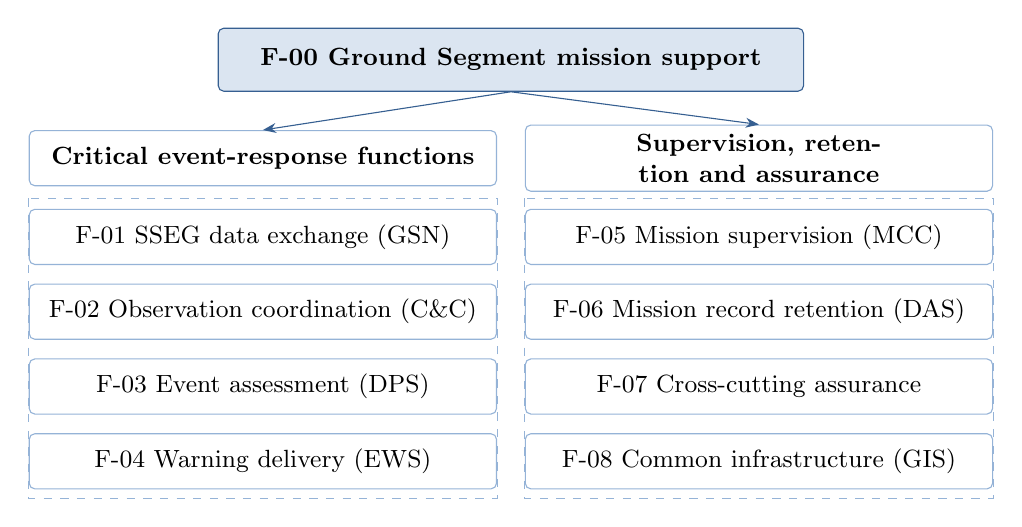
\begin{tikzpicture}[
  >=Stealth,
  root/.style={draw=HeadingBlue,fill=TableRowLightBlue,rounded corners=2pt,align=center,font=\bfseries\small,text width=7.2cm,minimum height=8mm},
  group/.style={draw=TableBorderBlue,fill=white,rounded corners=2pt,align=center,font=\bfseries\small,text width=5.7cm,minimum height=7mm},
  fn/.style={draw=TableBorderBlue,fill=white,rounded corners=2pt,align=center,font=\small,text width=5.7cm,minimum height=7mm},
  edge/.style={-Stealth,draw=HeadingBlue,thin}
]
\node[root] (root) at (0,0) {F-00 Ground Segment mission support};
\node[group] (critical) at (-3.15,-1.25) {Critical event-response functions};
\node[group] (support) at (3.15,-1.25) {Supervision, retention and assurance};
\node[fn] (f1) at (-3.15,-2.25) {F-01 SSEG data exchange (GSN)};
\node[fn] (f2) at (-3.15,-3.20) {F-02 Observation coordination (C\&C)};
\node[fn] (f3) at (-3.15,-4.15) {F-03 Event assessment (DPS)};
\node[fn] (f4) at (-3.15,-5.10) {F-04 Warning delivery (EWS)};
\node[fn] (f5) at (3.15,-2.25) {F-05 Mission supervision (MCC)};
\node[fn] (f6) at (3.15,-3.20) {F-06 Mission record retention (DAS)};
\node[fn] (f7) at (3.15,-4.15) {F-07 Cross-cutting assurance};
\node[fn] (f8) at (3.15,-5.10) {F-08 Common infrastructure (GIS)};
\draw[edge] (root.south) -- (critical.north);
\draw[edge] (root.south) -- (support.north);
\draw[draw=TableBorderBlue,dashed] (-6.13,-1.76) rectangle (-0.17,-5.57);
\draw[draw=TableBorderBlue,dashed] (0.17,-1.76) rectangle (6.13,-5.57);
\end{tikzpicture}
\caption{GSEG first-level function tree and functional groupings.}
\label{fig:gseg_function_tree}
\end{figure}

The allocation below defines the responsible subsystem at GSEG level; internal decomposition remains subject to the corresponding subsystem DDFs.

{\DDFTableStyle{3}%
\begin{longtable}{|L{0.14}|L{0.72}|L{0.14}|}
\caption{GSEG function allocation}\label{tab:gseg_function_allocation}\\
\hline\rowcolor{TableHeaderBlue}
\thead{ID} & \thead{Function} & \thead{Owner}\\\hline
\endfirsthead
\hline\rowcolor{TableHeaderBlue}\thead{ID} & \thead{Function} & \thead{Owner}\\\hline
\endhead
F-01.1 & Receive and route GEO Event Reports. & GSN\\ \hline
F-01.2 & Transfer LEO Tracking Requests to the SSEG interface. & GSN\\ \hline
F-01.3 & Receive and route LEO Observation Packages and the Onboard Preliminary Trajectory. & GSN\\ \hline
F-01.4 & Exchange spacecraft telemetry and communications status. & GSN\\ \hline
F-02.1 & Evaluate LEO observation opportunities and select two spacecraft. & C\&C\\ \hline
F-02.2 & Generate tracking requests and coordinate their handover. & C\&C\\ \hline
F-02.3 & Track command transmission and execution status. & C\&C\\ \hline
F-03.1 & Associate and validate observation inputs against the event record. & DPS\\ \hline
F-03.2 & Automatically classify valid assessments and determine warning eligibility; distinguish the separate Assessment Unavailable status. & DPS\\ \hline
F-03.3 & Fuse the two selected LEO observation sets and onboard preliminary trajectory. & DPS\\ \hline
F-03.4 & Produce refined trajectory, probabilistic impact area and uncertainty information. & DPS\\ \hline
F-03.5 & Prioritize Baltic-region threats and update assessments as new data arrive. & DPS\\ \hline
F-04.1 & Generate and automatically deliver the first preliminary warning only for warning-eligible outcomes, including the corresponding uncertainty. & EWS\\ \hline
F-04.2 & Track warning delivery status and available acknowledgements. & EWS\\ \hline
F-04.3 & Disseminate authorized post-warning confirmation, revision or cancellation. & EWS\\ \hline
F-05.1 & Present spacecraft and service status, all event-assessment outcomes and warning issue/non-issue decisions and reasons. & MCC\\ \hline
F-05.2 & Support authorized operator actions after first-warning delivery. & MCC\\ \hline
F-05.3 & Coordinate orbital-conjunction information for mission supervision and SSEG. & MCC\\ \hline
F-05.4 & Produce orbit predictions and mission plans for operational use, including current orbital products for C\&C. & MCC\\ \hline
F-06.1 & Record mission products, commands, classification or unavailable-assessment status, warning issue/non-issue decisions and reasons, warning history and audit information. & DAS\\ \hline
F-06.2 & Retain and provide authorized retrieval of mission history. & DAS\\ \hline
F-07.1 & Enforce access control and command authenticity at relevant functions. & Shared\\ \hline
F-07.2 & Protect information and preserve event/product traceability. & Shared\\ \hline
F-07.3 & Detect loss of critical services and support redundant functional paths. & Shared\\ \hline
F-08.1 & Provide shared compute and internal network infrastructure for GSEG services. & GIS\\ \hline
F-08.2 & Provide site power, cooling and common time-reference services. & GIS\\ \hline
F-08.3 & Monitor and maintain availability of common site infrastructure. & GIS\\ \hline
F-08.4 & Maintain shared execution capacity for concurrent critical event workflows. & GIS\\ \hline
\end{longtable}}

MCC owns the operational coordination of orbital-conjunction information (F-05.3). The physical ingress route and forwarding implementation are defined by the relevant interface design. Flight-dynamics products from MCC are made available for C\&C observation planning; their routine preparation and operator review do not gate automatic two-LEO selection after a GEO report. GIS provides enabling infrastructure, while security and mission-product traceability remain shared responsibilities across subsystems. DPS classification does not gate C\&C LEO selection.

\newpage
\subsection{4.3 Functional Chains and Operational States}

\subsubsection{4.3.1 Critical Warning Chain}

The critical chain consists of two GSEG processing intervals separated by SSEG tracking activities (Figure~\ref{fig:gseg_critical_chain}):

\begin{itemize}
\item \textbf{Observation tasking:} GSN receives the GEO report; C\&C selects two LEO spacecraft and prepares tracking requests for GSN handover (2~s maximum; \texttt{GSEG-REQ-PERF-001}).
\item \textbf{Assessment and conditional warning:} after GSN receives both required LEO Observation Packages and the Onboard Preliminary Trajectory, DPS validates the data, classifies the event and determines warning eligibility. For warning-eligible events, EWS automatically delivers the first preliminary warning at the authorized recipient interface (\texttt{GSEG-REQ-PERF-002}; 15~s maximum).
\end{itemize}

\begin{figure}[H]
\centering
\resizebox{0.98\linewidth}{!}{%
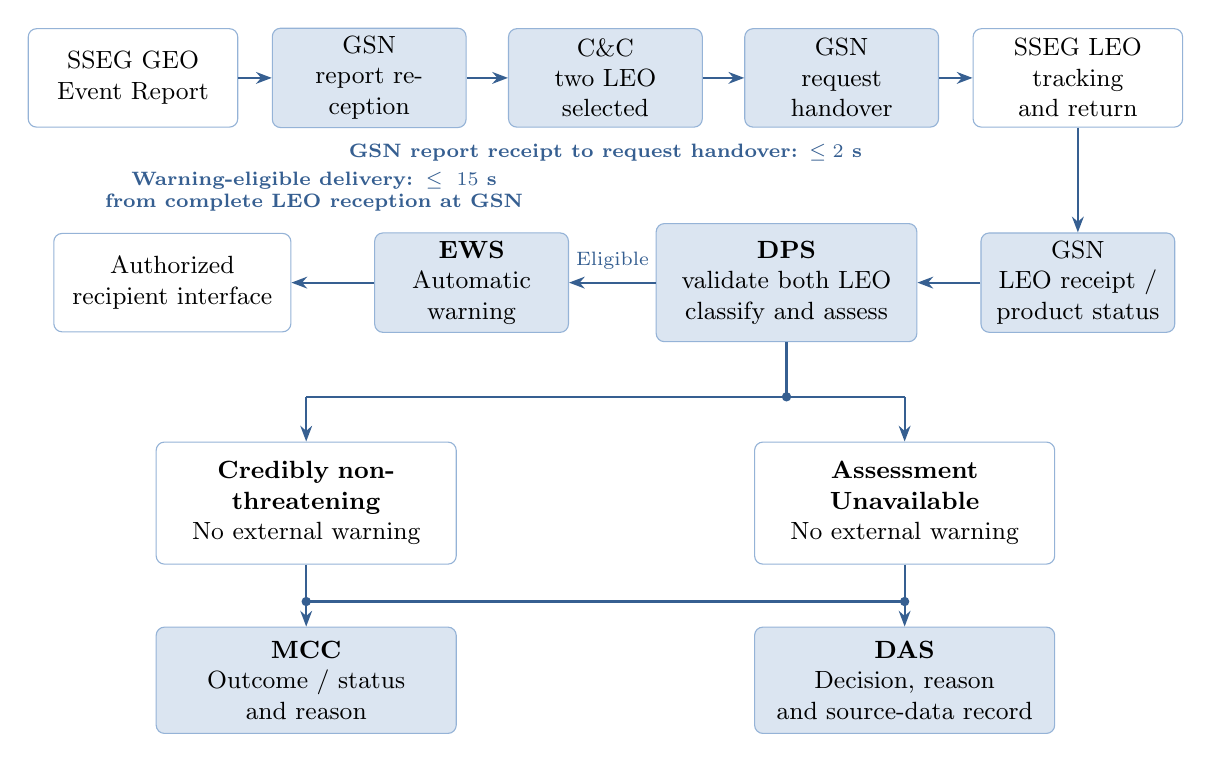
\begin{tikzpicture}[
  >=Stealth,
  stage/.style={draw=TableBorderBlue,fill=TableRowLightBlue,rounded corners=3pt,align=center,font=\small,text width=2.25cm,minimum height=1.25cm,inner sep=3pt},
  external/.style={stage,fill=white,text width=2.45cm},
  assess/.style={stage,text width=3.1cm,minimum height=1.50cm},
  outcome/.style={stage,fill=white,text width=3.6cm,minimum height=1.55cm},
  record/.style={stage,text width=3.6cm,minimum height=1.35cm},
  arrow/.style={-{Stealth[length=2mm]},draw=HeadingBlue,line width=0.8pt},
  link/.style={draw=HeadingBlue,line width=0.8pt},
  timing/.style={font=\scriptsize\bfseries,text=HeadingBlue,align=center},
  junction/.style={circle,fill=HeadingBlue,inner sep=1.2pt}
]
\node[external] (geo) at (-6,0) {SSEG GEO\\Event Report};
\node[stage] (gsnup) at (-3,0) {GSN\\report reception};
\node[stage] (cc) at (0,0) {C\&C\\two LEO selected};
\node[stage] (handover) at (3,0) {GSN\\request handover};
\node[external] (sseg) at (6,0) {SSEG LEO\\tracking and return};
\node[stage] (gsndown) at (6,-2.6) {GSN\\LEO receipt /\\product status};
\node[assess] (dps) at (2.3,-2.6) {\textbf{DPS}\\validate both LEO\\classify and assess};
\node[stage] (ews) at (-1.7,-2.6) {\textbf{EWS}\\Automatic\\warning};
\node[external,text width=2.8cm] (recipient) at (-5.5,-2.6) {Authorized\\recipient interface};
\node[outcome] (nonthreat) at (-3.8,-5.4) {\textbf{Credibly non-threatening}\\No external warning};
\node[outcome] (unavailable) at (3.8,-5.4) {\textbf{Assessment Unavailable}\\No external warning};
\node[record] (mcc) at (-3.8,-7.65) {\textbf{MCC}\\Outcome / status\\and reason};
\node[record] (das) at (3.8,-7.65) {\textbf{DAS}\\Decision, reason\\and source-data record};
\draw[arrow] (geo.east) -- (gsnup.west);
\draw[arrow] (gsnup.east) -- (cc.west);
\draw[arrow] (cc.east) -- (handover.west);
\draw[arrow] (handover.east) -- (sseg.west);
\draw[arrow] (sseg.south) -- (gsndown.north);
\draw[arrow] (gsndown.west) -- (dps.east);
\draw[arrow] (dps.west) -- (ews.east);
\node[font=\scriptsize,text=HeadingBlue,fill=white,inner sep=1pt] at (0.09,-2.32) {Eligible};
\draw[arrow] (ews.west) -- (recipient.east);
% DPS supplies one of the two no-warning outcomes; the decision table defines eligibility.
\draw[link] (dps.south) -- (2.3,-4.05);
\draw[link] (-3.8,-4.05) -- (3.8,-4.05);
\node[junction] at (2.3,-4.05) {};
\draw[arrow] (-3.8,-4.05) -- (nonthreat.north);
\draw[arrow] (3.8,-4.05) -- (unavailable.north);
% Both no-warning outcomes are reported to MCC and retained by DAS.
\draw[link] (nonthreat.south) -- (-3.8,-6.65);
\draw[link] (unavailable.south) -- (3.8,-6.65);
\draw[link] (-3.8,-6.65) -- (3.8,-6.65);
\foreach \x in {-3.8,3.8}{\node[junction] at (\x,-6.65) {};}
\draw[arrow] (-3.8,-6.65) -- (mcc.north);
\draw[arrow] (3.8,-6.65) -- (das.north);
\node[timing] at (0,-0.95) {GSN report receipt to request handover: $\leq 2$ s};
\node[timing,text width=6.1cm] at (-3.7,-1.45) {Warning-eligible delivery: $\leq 15$ s\\from complete LEO reception at GSN};
\end{tikzpicture}}
\caption[Conditional critical warning chain and DPS decision branches.]{Conditional critical warning chain. The 2 s interval runs from GSN report reception to tracking-request handover. The 15 s interval runs from complete required two-LEO product reception at GSN to authorized-interface delivery for warning-eligible events; SSEG tracking is outside both GSEG intervals. Both no-warning outcomes are reported to MCC and recorded in DAS. Dots denote connected branches.}
\label{fig:gseg_critical_chain}
\end{figure}

DPS distinguishes three threat classes for valid assessments and a separate data-validity status, \emph{Assessment Unavailable}. Table~\ref{tab:gseg_warning_decision} defines the integrated response; unavailability is not a fourth threat class.

{\DDFTableStyle{2}%
\begin{longtable}{|L{0.47}|L{0.53}|}
\caption{DPS assessment outcomes and conditional GSEG response}\label{tab:gseg_warning_decision}\\\hline
\rowcolor{TableHeaderBlue}\thead{DPS outcome} & \thead{Integrated GSEG response}\\\hline\endfirsthead
\hline\rowcolor{TableHeaderBlue}\thead{DPS outcome} & \thead{Integrated GSEG response}\\\hline\endhead
\texttt{POTENTIAL\_THREAT}\newline Valid two-LEO assessment; refined trajectory and impact-area estimate. & EWS automatically delivers the first preliminary warning to the authorized recipient interface.\\\hline
\texttt{INDETERMINATE\_\allowbreak CREDIBLE\_\allowbreak THREAT\_\allowbreak NOT\_\allowbreak EXCLUDED}\newline Valid assessment; a credible threat cannot be excluded. & EWS automatically delivers the first preliminary warning with explicit uncertainty information.\\\hline
\texttt{CREDIBLY\_\allowbreak NON\_\allowbreak THREATENING}\newline Valid assessment; a credible threat is excluded. & No external warning. MCC receives the result and reason; DAS retains the decision, reason and source data.\\\hline
\texttt{ASSESSMENT\_\allowbreak UNAVAILABLE}\newline Missing, invalid or insufficient required observations or products. & No external warning. Report inability to assess to MCC; retain the status and reason in DAS.\\\hline
\end{longtable}}

Under \texttt{GSEG-REQ-FUN-005}, the first warning requires valid assessment of both selected LEO observation sets, a refined ground trajectory and an impact-area estimate, and a potential threat or an indeterminate assessment for which a credible threat cannot be excluded. DPS determines the classification and warning eligibility; EWS distributes the warning. MCC review and DAS write completion do not gate the first warning. Thresholds distinguishing credible threats and non-threatening events remain TBD for DPS/EWS design and DDJF substantiation; no numerical decision threshold is established here.

\subsubsection{4.3.2 Supporting and Update Chains}

C\&C, GSN, DPS and EWS provide relevant operational and event status to MCC, including all classification and warning-decision outcomes. DAS records applicable mission products, commands, warning issue/non-issue decisions and reasons, warning versions and audit information in parallel with the critical chain. New observations trigger updated DPS assessments; an authorized operator may subsequently confirm, revise or cancel an issued warning through MCC and EWS.

\subsubsection{4.3.3 Operational States and Degraded Operation}

\begin{itemize}
\setlength{\itemsep}{0pt}
\setlength{\parsep}{0pt}
\setlength{\parskip}{0pt}
\item \textbf{Nominal monitoring:} constellation and ground-service supervision, with event-response functions ready.
\item \textbf{Event response:} GEO report reception, LEO selection and tracking-request handover.
\item \textbf{Event assessment:} receipt and validation of LEO products, classification and ground fusion.
\item \textbf{Warning dissemination, for eligible events:} automatic delivery of the first preliminary warning.
\item \textbf{Post-warning operations:} updated assessments, operator actions and warning updates.
\end{itemize}

These are event stages, not mutually exclusive GSEG modes. Assessment Unavailable produces no external warning and status/records for MCC/DAS; service loss is reported to MCC. Ten concurrent events are a proposed sizing case (P), not a mission maximum. MCC prepares orbital products in advance; C\&C selection does not wait for DPS classification, fresh flight-dynamics computation or operator approval. Physical recovery is defined outside Section~4.

\section{5. Physical Description}\label{physical-description}

\subsection{5.1 Physical Architecture}\label{physical-architecture}

GSEG is located at one geographical site (\texttt{GSEG-\allowbreak{}REQ-\allowbreak{}ARC-\allowbreak{}001}). It
comprises GSN as a separate satellite-communications layer, C\&C, DPS
and EWS services, mission supervision and Flight Dynamics (MCC), the
archive (DAS) and shared GIS infrastructure.

The GIS platform provides logical separation between critical services
and archival and operator workloads. The preliminary architecture
assumes two separate equipment failure domains, each with the
resources required to accommodate the full critical-service load
following the loss of the other domain. This is a capacity allocation
(P), not demonstrated failover effectiveness. GSN RF equipment and MCC
workstations remain physically separated from the shared compute hosts.

\begin{figure}[H]
\centering
% Logical equipment groups and exchanges from DDF 5.5.1--5.5.2.
% Named source sets summarize independent logical inputs, not extra hardware.
\resizebox{0.98\linewidth}{!}{%
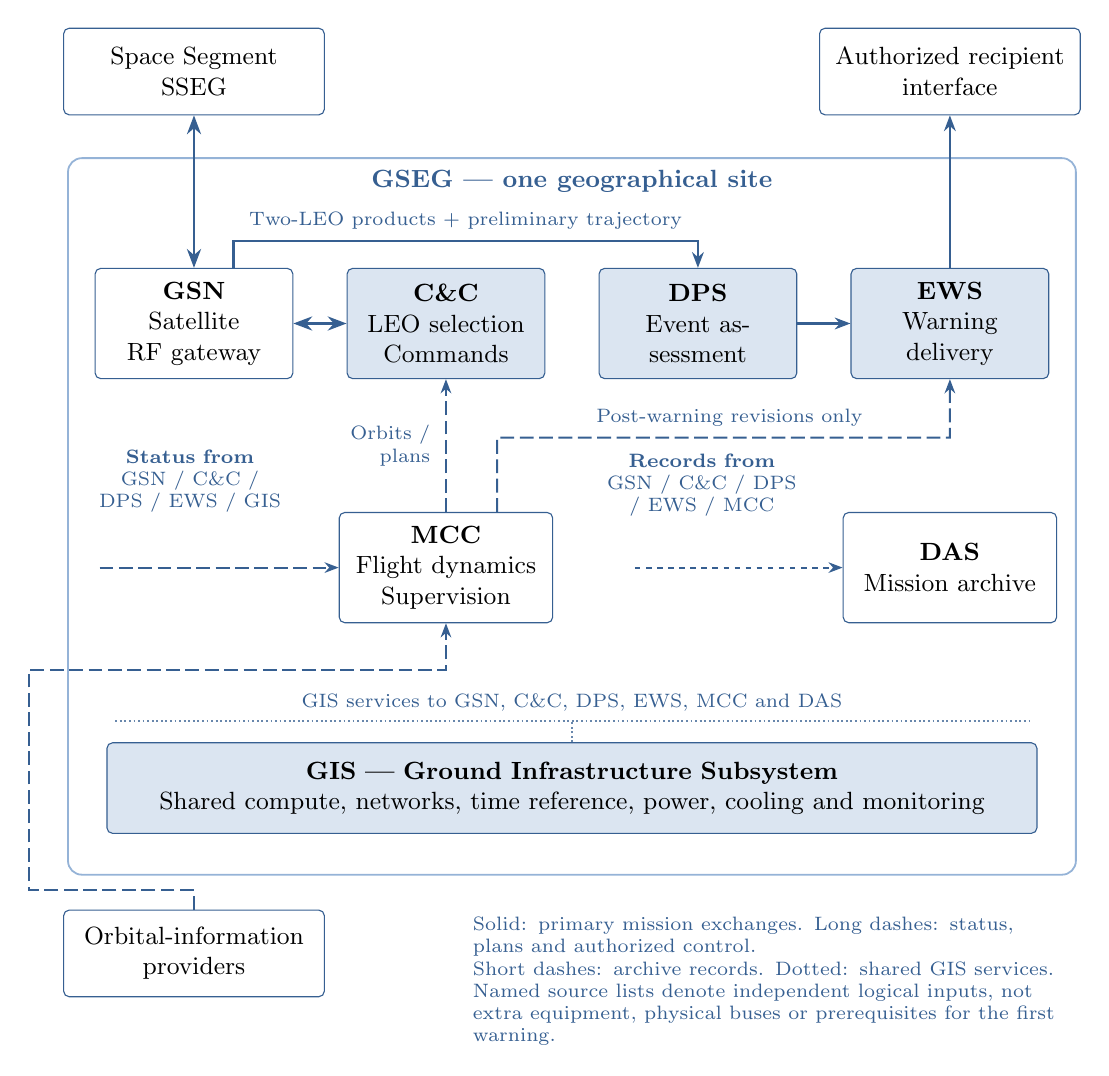
\begin{tikzpicture}[
  >=Stealth,
  gsegEquipment/.style={draw=HeadingBlue,fill=TableRowLightBlue,
    rounded corners=2pt,align=center,font=\small,text width=2.3cm,
    minimum height=1.4cm,inner sep=3pt},
  gsegSupport/.style={gsegEquipment,fill=white,text width=2.5cm},
  gsegExternal/.style={gsegEquipment,fill=white,text width=3.1cm,
    minimum height=1.1cm},
  gsegInfrastructure/.style={gsegEquipment,text width=11.6cm,
    minimum height=1.15cm},
  gsegMission/.style={draw=HeadingBlue,line width=0.85pt},
  gsegData/.style={gsegMission,-{Stealth[length=2mm]}},
  gsegOperations/.style={draw=HeadingBlue,dash pattern=on 5pt off 2pt,
    line width=0.7pt,-{Stealth[length=1.8mm]}},
  gsegArchive/.style={draw=HeadingBlue,dash pattern=on 2pt off 2pt,
    line width=0.7pt,-{Stealth[length=1.8mm]}},
  gsegServices/.style={draw=HeadingBlue!75,densely dotted,line width=0.65pt},
  gsegChannelLabel/.style={align=center,font=\scriptsize,text=HeadingBlue,
    inner sep=1pt},
  gsegNote/.style={align=left,font=\scriptsize,text=HeadingBlue,inner sep=1pt}
]
% One geographical site, containing exactly the seven GSEG subsystems.
\draw[draw=TableBorderBlue,rounded corners=5pt,line width=0.65pt]
  (-6.4,-3.0) rectangle (6.4,6.1);
\node[font=\small\bfseries,text=HeadingBlue] at (0,5.8)
  {GSEG --- one geographical site};

\node[gsegExternal] (sseg) at (-4.8,7.2) {Space Segment\\SSEG};
\node[gsegExternal] (recipient) at (4.8,7.2)
  {Authorized recipient\\interface};
\node[gsegEquipment,fill=white] (gsn) at (-4.8,4.0)
  {\textbf{GSN}\\Satellite RF gateway};
\node[gsegEquipment] (cc) at (-1.6,4.0)
  {\textbf{C\&C}\\LEO selection\\Commands};
\node[gsegEquipment] (dps) at (1.6,4.0)
  {\textbf{DPS}\\Event assessment};
\node[gsegEquipment] (ews) at (4.8,4.0)
  {\textbf{EWS}\\Warning delivery};

% Primary mission exchanges. There is no C&C -> DPS substitute path.
\draw[gsegMission,Stealth-Stealth] (sseg.south) -- (gsn.north);
\draw[gsegMission,Stealth-Stealth] (gsn.east) -- (cc.west);
\draw[gsegData] ($(gsn.north)+(0.5,0)$)
  -- (-4.3,5.05) -- (1.6,5.05) -- (dps.north);
\node[gsegChannelLabel,text width=6.0cm] at (-1.35,5.3)
  {Two-LEO products + preliminary trajectory};
\draw[gsegData] (dps.east) -- (ews.west);
\draw[gsegData] (ews.north) -- (recipient.south);

\node[gsegSupport] (mcc) at (-1.6,0.9)
  {\textbf{MCC}\\Flight dynamics\\Supervision};
\node[gsegSupport] (das) at (4.8,0.9)
  {\textbf{DAS}\\Mission archive};

% Precomputed plans/orbits and later warning revisions use separate routes.
\draw[gsegOperations] (mcc.north) -- (cc.south);
\node[gsegChannelLabel,align=right,text width=1.1cm] at (-2.35,2.45)
  {Orbits /\\plans};
\draw[gsegOperations] ($(mcc.north)+(0.65,0)$)
  -- (-0.95,2.55) -- (4.8,2.55) -- (ews.south);
\node[gsegChannelLabel,text width=4.0cm] at (2.0,2.8)
  {Post-warning revisions only};

% Independent source lists explicitly define the logical collection channels.
% No collection channel is shown as a new subsystem or as routing through MCC.
\node[gsegChannelLabel,text width=2.75cm] at (-4.85,2.0)
  {\textbf{Status from}\\GSN / C\&C / DPS / EWS / GIS};
\draw[gsegOperations] (-6.0,0.9) -- (mcc.west);
\node[gsegChannelLabel,text width=3.4cm] at (1.65,1.95)
  {\textbf{Records from}\\GSN / C\&C / DPS / EWS / MCC};
\draw[gsegArchive] (0.8,0.9) -- (das.west);

% Shared infrastructure is a provider layer, never a warning-processing stage.
\node[gsegInfrastructure] (gis) at (0,-1.9)
  {\textbf{GIS --- Ground Infrastructure Subsystem}\\
   Shared compute, networks, time reference, power, cooling and monitoring};
\draw[gsegServices] (gis.north) -- (0,-1.05);
\draw[gsegServices] (-5.8,-1.05) -- (5.8,-1.05);
\node[gsegChannelLabel,text width=11.6cm] at (0,-0.82)
  {GIS services to GSN, C\&C, DPS, EWS, MCC and DAS};

% Orbital-information providers are external; the entry point is MCC.
\node[gsegExternal] (orbital) at (-4.8,-4.0)
  {Orbital-information\\providers};
\draw[gsegOperations] (orbital.north) -- (-4.8,-3.2)
  -- (-6.9,-3.2) -- (-6.9,-0.4) -- (-1.6,-0.4) -- (mcc.south);

\node[gsegNote,anchor=north west,text width=7.4cm] at (-1.3,-3.5) {
  Solid: primary mission exchanges. Long dashes: status, plans and authorized control.\\
  Short dashes: archive records. Dotted: shared GIS services.\\
  Named source lists denote independent logical inputs, not extra equipment,
  physical buses or prerequisites for the first warning.};
\end{tikzpicture}%
}

\caption{Figure 5-1. GSEG equipment groups and logical relationships.
Solid lines: principal mission products; dashed: supervision and
archiving; dotted: GIS support. The diagram does not define wiring or RF
redundancy.}
\end{figure}

EWS is the sole path for delivering warnings to authorized recipients.
MCC may initiate later updates but sends them to EWS, not directly to
the recipient.

Required availability boundary: the 99.99\% assessment includes
GSN RF equipment and ground gateways, GIS, and GSEG-controlled
connections and warning-delivery interfaces. Independent failures of
SSEG spacecraft or recipient systems \emph{beyond the agreed interface
boundary} are not counted against GSEG availability. The single site
remains a common-cause failure exposure that is not removed by dividing
GIS into two domains.

\subsection{5.2 Product Tree}\label{product-tree}

The product tree defines seven GSEG subsystems and five subordinate
product items: two within DAS and three within DPS. The GIS product
identifier is \texttt{123456.02.07}.

\begin{figure}[H]
\centering
% Seven subsystem nodes, with exactly two DAS and three DPS product nodes.
\resizebox{0.98\linewidth}{!}{%
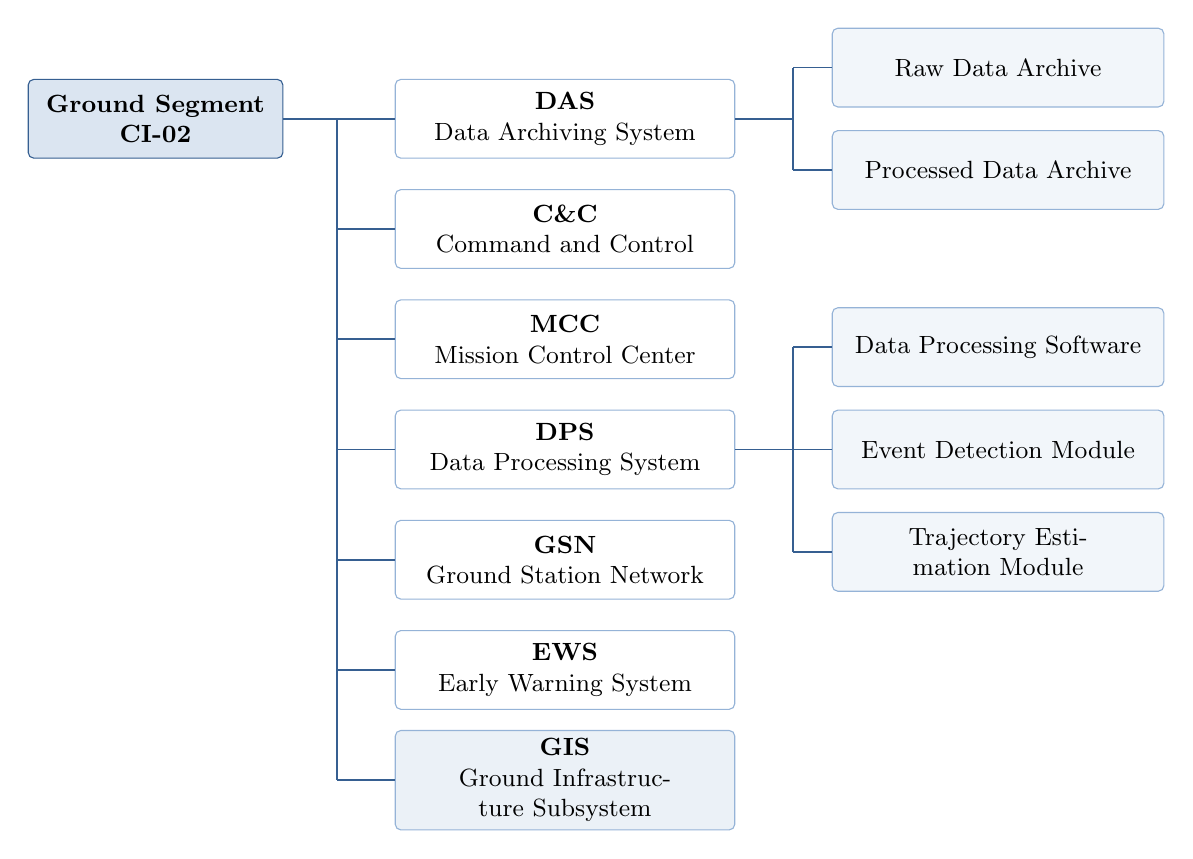
\begin{tikzpicture}[
  root/.style={draw=HeadingBlue,fill=TableRowLightBlue,rounded corners=2pt,
    align=center,font=\small\bfseries,text width=3.0cm,minimum height=1.0cm},
  item/.style={draw=TableBorderBlue,fill=white,rounded corners=2pt,
    align=center,font=\small,text width=4.1cm,minimum height=1.0cm,inner sep=3pt},
  product/.style={item,fill=TableRowLightBlue!35,text width=4.0cm},
  link/.style={draw=HeadingBlue,line width=0.65pt}
]
\node[root] (gseg) at (-5.7,0) {Ground Segment\\CI-02};
\node[item] (das) at (-0.5,0) {\textbf{DAS}\\Data Archiving System};
\node[item] (cc) at (-0.5,-1.4) {\textbf{C\&C}\\Command and Control};
\node[item] (mcc) at (-0.5,-2.8) {\textbf{MCC}\\Mission Control Center};
\node[item] (dps) at (-0.5,-4.2) {\textbf{DPS}\\Data Processing System};
\node[item] (gsn) at (-0.5,-5.6) {\textbf{GSN}\\Ground Station Network};
\node[item] (ews) at (-0.5,-7.0) {\textbf{EWS}\\Early Warning System};
\node[item,fill=TableRowLightBlue!55] (gis) at (-0.5,-8.4)
  {\textbf{GIS}\\Ground Infrastructure Subsystem};
\draw[link] (gseg.east) -- (-3.4,0) -- (-3.4,-8.4);
\foreach \name in {das,cc,mcc,dps,gsn,ews,gis} {
  \draw[link] (-3.4,0 |- \name.west) -- (\name.west);
}
\node[product] (raw) at (5.0,0.65) {Raw Data Archive};
\node[product] (processed) at (5.0,-0.65) {Processed Data Archive};
\draw[link] (das.east) -- (2.4,0);
\draw[link] (2.4,0.65) -- (2.4,-0.65);
\draw[link] (2.4,0.65) -- (raw.west);
\draw[link] (2.4,-0.65) -- (processed.west);
\node[product] (software) at (5.0,-2.9) {Data Processing Software};
\node[product] (detection) at (5.0,-4.2) {Event Detection Module};
\node[product] (trajectory) at (5.0,-5.5) {Trajectory Estimation Module};
\draw[link] (dps.east) -- (2.4,-4.2);
\draw[link] (2.4,-2.9) -- (2.4,-5.5);
\foreach \name in {software,detection,trajectory} {
  \draw[link] (2.4,0 |- \name.west) -- (\name.west);
}
\end{tikzpicture}%
}

\caption{Figure 5-2. GSEG product tree: seven subsystems and
five separate DAS and DPS product items.}
\end{figure}

The subordinate DAS elements are Raw Data Archive and
Processed Data Archive. The subordinate DPS elements are
Data Processing Software, Event Detection Module and
Trajectory Estimation Module. Their respective WBS identifiers
remain \texttt{123456.02.01.01}, \texttt{.01.02}, \texttt{.04.01},
\texttt{.04.02} and \texttt{.04.03}.

\subsection{5.3 Specification Tree}\label{specification-tree}

The GSEG TRS (\texttt{EWAS-\allowbreak{}HSB-\allowbreak{}GSEG-\allowbreak{}TRS-\allowbreak{}02}) is the parent specification
for seven planned subsystem TRSs. Subsystem TRSs have not yet been
issued. DDFs and DDJFs define and justify the design, but are not
branches of the \emph{requirements specification tree}; agreed
interfaces are controlled in ICDs.

\begin{figure}[H]
\centering
% Requirements hierarchy only; no DDF or DDJF branches.
\resizebox{0.98\linewidth}{!}{%
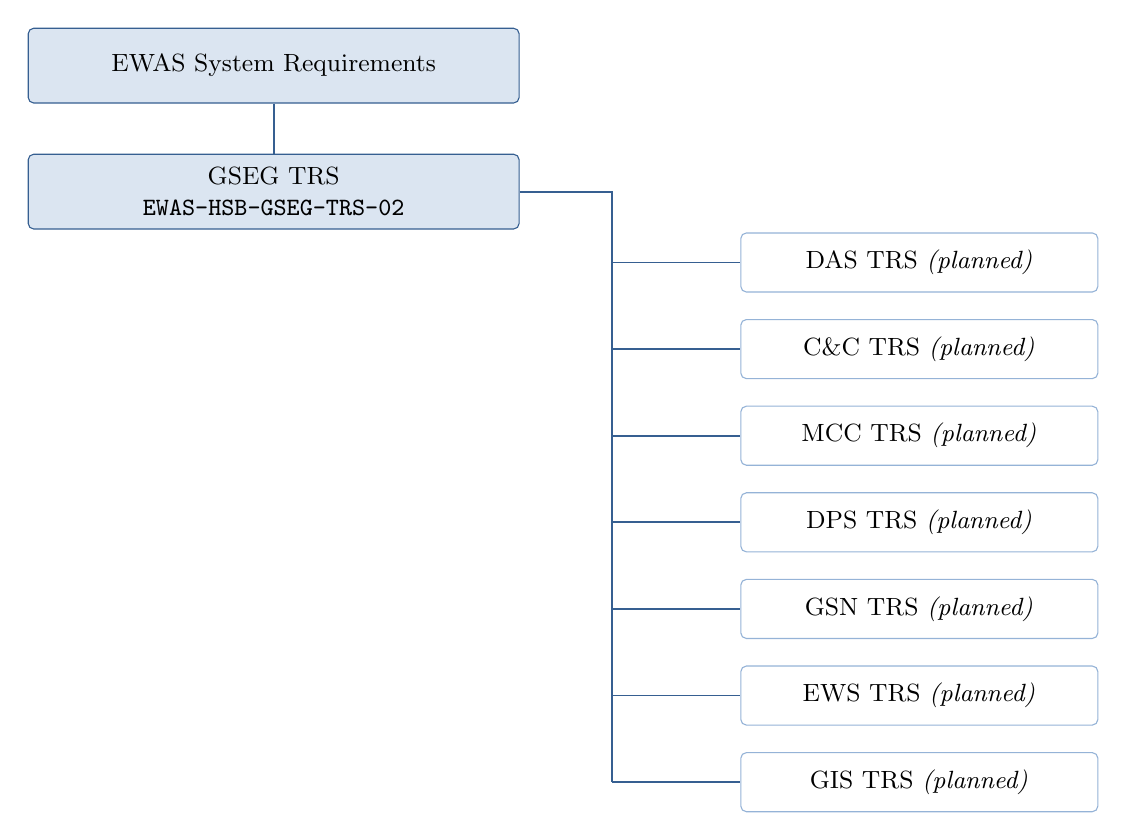
\begin{tikzpicture}[
  parent/.style={draw=HeadingBlue,fill=TableRowLightBlue,rounded corners=2pt,
    align=center,font=\small,text width=6.0cm,minimum height=0.95cm},
  child/.style={draw=TableBorderBlue,fill=white,rounded corners=2pt,
    align=center,font=\small,text width=4.3cm,minimum height=0.75cm},
  link/.style={draw=HeadingBlue,line width=0.65pt}
]
\node[parent] (system) at (-3.8,0) {EWAS System Requirements};
\node[parent] (gseg) at (-3.8,-1.6)
  {GSEG TRS\\\texttt{EWAS-HSB-GSEG-TRS-02}};
\draw[link] (system.south) -- (gseg.north);
\node[child] (das) at (4.4,-2.5) {DAS TRS \textit{(planned)}};
\node[child] (cc) at (4.4,-3.6) {C\&C TRS \textit{(planned)}};
\node[child] (mcc) at (4.4,-4.7) {MCC TRS \textit{(planned)}};
\node[child] (dps) at (4.4,-5.8) {DPS TRS \textit{(planned)}};
\node[child] (gsn) at (4.4,-6.9) {GSN TRS \textit{(planned)}};
\node[child] (ews) at (4.4,-8.0) {EWS TRS \textit{(planned)}};
\node[child] (gis) at (4.4,-9.1) {GIS TRS \textit{(planned)}};
\draw[link] (gseg.east) -- (0.5,-1.6) -- (0.5,-9.1);
\foreach \name in {das,cc,mcc,dps,gsn,ews,gis} {
  \draw[link] (0.5,0 |- \name.west) -- (\name.west);
}
\end{tikzpicture}%
}

\caption{Figure 5-3. GSEG requirements specification hierarchy.}
\end{figure}

\subsection{5.4 Physical Elements and Redundancy
Boundaries}\label{physical-elements-and-redundancy-boundaries}

\textbf{GSN --- communications layer.} Antennas, RF equipment and
link-handling equipment are physically separated from the managed
computing platform. The antenna configuration, radio redundancy and
demonstration of visibility and connectivity from one site remain within
the GSN DDF and system analyses.

\textbf{GIS --- shared infrastructure.} GIS is responsible for compute
hosts, networks and switches, common time, power, cooling and technical
monitoring. It hosts critical C\&C/DPS/EWS services in two equipment
domains, separated from DAS/MCC workloads. Each domain must provide the
full critical capacity after loss of the other. Host counts, state
replication, failover details and physical separation are to be designed
at lower levels. The site itself remains a common failure domain.

\textbf{MCC and DAS --- non-critical equipment.} MCC uses separate
operator workstations, while DAS archiving workloads are separated from
compute resources used by the critical warning chain. Both subsystems
use shared GIS services.

\subsection{5.5 Interfaces}\label{interfaces}

\subsubsection{5.5.1 External Interfaces}\label{external-interfaces}

\begingroup\GSEGTableStyle{3}
\begin{longtable}[]{|P{0.25}|P{0.19}|P{0.56}|}
\hline\rowcolor{TableHeaderBlue}
\begin{minipage}[b]{\linewidth}\raggedright
\color{white}\bfseries\sffamily
Boundary
\end{minipage} & \begin{minipage}[b]{\linewidth}\raggedright
\color{white}\bfseries\sffamily
GSEG owner
\end{minipage} & \begin{minipage}[b]{\linewidth}\raggedright
\color{white}\bfseries\sffamily
Exchanged products
\end{minipage} \\
\hline
\endhead
\hline
\endlastfoot
GSEG--SSEG (\texttt{IF-\allowbreak{}EXT-\allowbreak{}01}) & GSN & Commands, telemetry, GEO
reports, LEO packages and the onboard preliminary trajectory. \\ \hline
Authorized warning recipients & EWS & First warnings, revisions,
cancellations, status and available acknowledgements. \\ \hline
Orbital-data providers & MCC (operational ownership) & Predictions,
orbital and conjunction data; onward transmission to SSEG through C\&C
and GSN, taking \texttt{IF-\allowbreak{}EXT-\allowbreak{}04} into account. \\*
\end{longtable}
\endgroup

The physical ingress point for orbital data, the external connection
topology and protocol details require controlled ICDs. The ISL network
belongs to SSEG; its mere presence does not demonstrate communications
availability from a single GSEG site.

\subsubsection{5.5.2 Internal Interfaces}\label{internal-interfaces}

\begingroup\GSEGTableStyle{2}
\begin{longtable}[]{|P{0.31}|P{0.69}|}
\hline\rowcolor{TableHeaderBlue}
\begin{minipage}[b]{\linewidth}\raggedright
\color{white}\bfseries\sffamily
Relationship
\end{minipage} & \begin{minipage}[b]{\linewidth}\raggedright
\color{white}\bfseries\sffamily
Main products or services
\end{minipage} \\
\hline
\endhead
\hline
\endlastfoot
GSN ↔ C\&C & GEO reports, LEO requests, authenticated commands,
orbital-data forwarding packages, and command/link status. \\ \hline
GSN → DPS & LEO Observation Packages, onboard preliminary trajectory and
reception metadata. \\ \hline
DPS → EWS & Refined trajectory, impact-area assessment, uncertainty and
the event qualification outcome for warning; a warning is
dispatched only for a qualifying outcome. \\ \hline
GSN / C\&C / DPS / EWS / GIS → MCC & Spacecraft, command, service and
event status, classification and warning-decision outcome, and
infrastructure status. \\ \hline
MCC → C\&C & Current orbital data, conjunction assessments, approved
plans and operational directives. \\ \hline
MCC → EWS & Authorized requests for confirmation, revision or
cancellation. \\ \hline
GSN / C\&C / DPS / EWS / MCC → DAS & Mission products, event history,
\textbf{decisions to issue or withhold warnings}, warning versions and
audit data. \\ \hline
GIS → other GSEG subsystems & Compute, networking, time, power, cooling
and infrastructure management. \\*
\end{longtable}
\endgroup

These relationships are logical and do not define distinct cables or
protocols. Data schemas, security boundaries, data rates and error
handling are governed by the relevant ICDs and subsystem TRSs.

\textbf{Common time-base consistency:} the applicable SSEG specification
provides UTC timestamps in observation products
(\texttt{SSEG-\allowbreak{}REQ-\allowbreak{}FUN-\allowbreak{}006}) and spacecraft time synchronization
(\texttt{SSEG-\allowbreak{}REQ-\allowbreak{}ADCS-\allowbreak{}004}). GSEG retains the observation timestamp
received from SSEG and distinguishes it from the GSN product-reception
time, which marks the GSEG latency-budget boundary. GIS provides common
time services. Timestamp encoding on individual interfaces and allowable
correlation error remain subject to ICD agreement and the accuracy
budget; \textbf{the 50 µs accuracy specified for SSEG is not assigned to
GSEG}.


% Sections 6--9 will be added after their content is supplied and reviewed.

\end{document}
